% \section{Visuelle Grundstrukturen}

Ein wichtiger Faktor für den Erfolg des Scrum-Teams ist es, dass jeder im Team das gleiche Verständnis über das zu entwickelnde Produkt hat. Die Sicherstellung dessen ist von hoher Bedeutung, um vermeidbaren Zeitfressern, wie lange Diskussionen, Missverständnisse, Nacharbeit und eine \ggf daraus hervorgehende Demotivation im Team entgegenzuwirken.
Darüber hinaus entstehen durch eine Visualisierung des Produktes Ideen und Lösungsansätze für Abläufe und Features, die frühzeitig im Entwicklungsprozess angesprochen, diskutiert und eingearbeitet werden können, ohne einen bemerkbaren Mehraufwand zu generieren.
Wireframes eignen sich für diese Aufgabe sehr gut, da sich diese schnell erstellen und abändern lassen und zugleich jedem Teammitglied einen ersten Entwurf des Produktes aufzeigen. Ein weiterer Vorteil besteht darin, dass bereits frühzeitig dem Kunden auf einfache Weise die ersten Designkonzepte vorgestellt werden können und dieser sein Feedback in einer frühen Entwicklungsphase mit einfließen lassen kann.

Das Erstellen von Wireframes beinhaltet zugleich, sich frühzeitig mit dem Aufbau und der Konzeption der Website auseinanderzusetzen. Aus diesem Grunde wird im weiteren Verlauf auch auf die Themen Seitenstruktur und Layout eingegangen.

\subsection{Grundlagen Seitenstruktur}

Die Seitenstruktur einer Website beschreibt die Art und Weise, wie die Inhalte einer Anwendung präsentiert, organisiert und verlinkt sind.

Die darzustellenden Informationen müssen daher nach Inhalt aufgeteilt und thematisch auf einzelnen Seiten organisiert werden. Jede Seite der Website besitzt somit ein klares Ziel, worüber sie informieren soll. Die einzelnen Seiten unterscheiden sich daher \bzgl ihres Ziels und Inhaltes. Jedoch existieren auf jeder Website eine Reihe von sogenannten Kernseiten, die oft aufzufinden sind. Klassische Seitentypen sind \bspw Startseite, Kontaktseite, Landingpage, Content- sowie Detailseiten.

Die Startseite, auch als Homepage bekannt, beschreibt die Seite, die den Startpunkt \bzw Ursprung einer Website darstellt. Von ihr aus kann über Verlinkungen zu allen Unterseiten navigiert werden.
Die Landingpage hingegen ist die erste Seite, die ein User wahrnimmt, wenn er von einem externen Link auf die Website geführt wird und eine Session beginnt. Die Landingpage wird oft für das Marketing hergezogen, um den Besucher für den Dienst zu begeistern und weitere Schritte anzuregen.
Die Contentseite hingegen gibt einen Überblick über die angebotenen Inhalte und verweist auf die zugehörige Detailseite, auf der die Inhalte detailliert aufgeführt sind.

Wie aus der Beschreibung der Seitentypen hervorgeht, werden die einzelnen Seiten zu unterschiedlichen Zeitpunkten oder in einer bestimmten Reihenfolge aufgerufen. Dies lässt sich auch als eine Art Hierarchie verstehen, die die einzelnen Seiten zueinander haben. Ob es sich hierbei um eine flache oder tiefe Hierarchie handelt, ist von der Navigationsstruktur abhängig. Allgemein werden häufig, wegen der besseren Orientierung, flache Seitenhierarchien empfohlen.

\begin{figure}
    \centering
    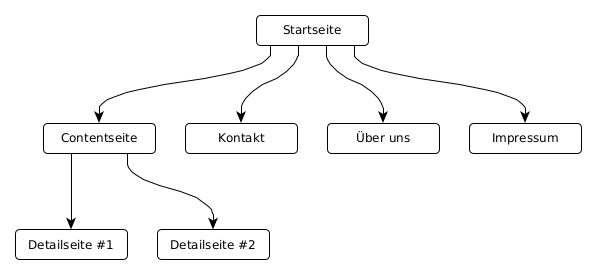
\includegraphics[width=\textwidth]{figures/jan/Wire_Hierarchie.png}
    \caption[Seitenstruktur einer Website]{Seitenstruktur einer Website}
    \label{fig:image}
\end{figure}

Die einzelnen Seiten einer Website unterscheiden sich jedoch \idR nicht vollständig voneinander. Sie folgen alle einem gleichbleibenden Aufbau. Dieses Grundgerüst einer Seite besteht oftmals aus einer Kopf- und Fußleiste und einem Inhaltsbereich. Die Kopf- und Fußleiste ist üblicherweise auf allen Seiten gleich ausgestaltet.

\begin{figure}
    \centering
    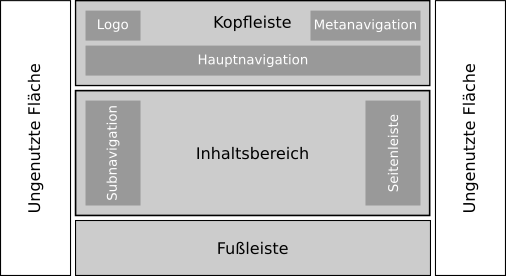
\includegraphics[]{figures/jan/Wire_Areas.png}
    \caption[Elemente einer Website]{Elemente einer Website}
    \label{fig:image}
\end{figure}

Der Kopfbereich einer Seite befindet sich im obersten Teil der Seite und umfasst das Logo, die Haupt- und Metanavigation. Der Kopfbereich wird häufig auch als Header bezeichnet.
Das Logo im Kopfbereich stellt ein wichtiges Erkennungs- und Differenzierungsmerkmal der Website dar und zielt auf das Erzeugen von Assoziationen mit der Website ab. Die Hauptnavigation gibt eine Übersicht über die verfügbaren Inhalte und stellt diese strukturiert dar. Die Hauptnavigation erweist sich für die Navigation als wichtigstes Element und wird häufig auffällig im oberen Bereich platziert. Eine weitere Navigationsleiste ist die Metanavigation, welche ergänzende Serviceinhalte wie \zB Accounteinstellungen der Seite verfügbar macht. Die Inhalte dieser Leiste haben keinen Bezug zu den Hauptthemen und werden daher gesondert aufgeführt.

Der Inhaltsbereich ist direkt unter dem Kopfbereich angeordnet und umfasst die zu vermittelnden Inhalte. Der Inhaltsbereich weist je nach Bedarf entweder nur die reinen Inhalte auf oder \ggf noch eine Subnavigation, die meist links angeordnet ist, sowie eine Seitenleiste (\engl Sidebar) für weiterführende Inhalte, die auf der rechten Seite untergebracht werden. Die zentralen Inhalte werden zwischen den Leisten, im sogenannten Inhaltsbereich, und meist nach Wichtigkeit absteigend sortiert aufgelistet.

Die untere Begrenzung der Internetseite bildet die Fußleiste (\engl Footer). Die Fußleiste beinhaltet meist Basisinformationen der Seite, ergänzende Inhalte oder auch \ggf weitere Navigationsmöglichkeiten.

Umschlossen werden die Seitenbereiche von einem umgebenden Block, der die ungenutzte Fläche der Website darstellt.

\subsection{Grundlagen Layout}
\subsection{Rastersystem}

Für die Überführung der ersten Skizzen in ein stimmiges Layout eignet sich die zur Hilfenahme eines Rastersystems. Ein Rastersystem stellt ein Netz mit Zeilen und Spalten dar, an welchen die Inhalte ausgerichtet und letztlich im Rastersystem platziert werden. Der Vorteil besteht darin, dass die Inhaltselemente und Einzelseiten in eine gleiche Struktur gebracht werden und die Seiten zunehmend abgestimmter und einheitlicher wirken. Das Raster wird lediglich für die Gestaltung herangezogen und sollte möglichst unauffällig oder dezent für den Endnutzer wirken,

Die Ausgangsbasis eines Rastersystems ist zu meist eine Leinwand mit definierten Abmessungen. Die Fläche wird in Spalten (\engl columns) unterteilt und \ggf wird zusätzlich noch zwischen den Spalten ein gleichbleibender Freiraum (\engl gutter) angelegt. Je höher die Spaltenanzahl gewählt wird, desto größer wird der gestalterische Spielraum, wobei der Nutzen des Rasters ab einer gewissen Anzahl zunehmend verschwindet.
In einem weiteren Schritt kann eine horizontale Unterteilung vorgenommen werden. Als Grundlage wird hier das sogenannte Baseline Grid verwendet, welches sich aus der Schriftgröße und dem Zeilenabstand zusammensetzt.
Die einzelnen Spalten und Zeilen können des Weiteren noch in Bereiche zusammengefasst werden, um ein modulares Rastersystem zu erstellen.
Die Website-Inhalte werden im Nachgang den Bereich zugeordnet und am Raster ausgerichtet.

\begin{figure}
    \centering
    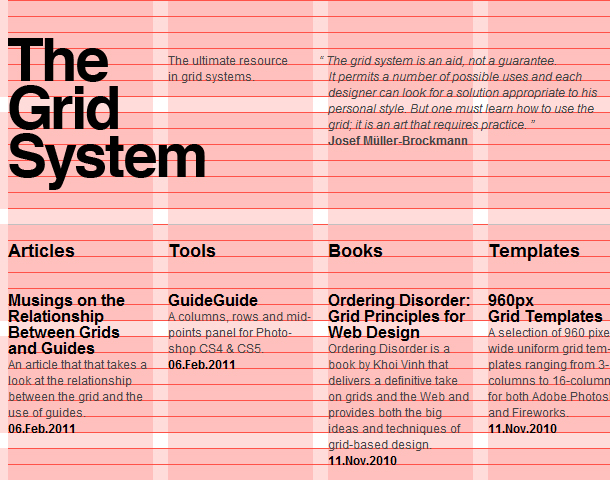
\includegraphics[width=0.6\textwidth]{figures/jan/Wire_Gridsystem.jpeg}
    \caption[Beispiel eines Rastersystems]{Beispiel eines Rastersystems}
    \label{fig:image}
\end{figure}

% ![Gridsystem](res/Wire_Gridsystem.jpeg)
% [//]: # (BILD Gridsystem: https://www.elmastudio.de/wp-content/uploads/2011/02/rastersysteme-webdesign-07.jpg)

\subsubsection*{Layouttypen}

Als es nur eine kleine Vielfalt an Endgeräten mit verschiedenen Auflösungen gab, wurde oft mit einem statischen Layout gearbeitet, welches für eine weit verbreitete Auflösung optimiert war. Heute lässt sich dieser Ansatz wegen der unüberschaubaren Menge an Geräten, die sich zudem stark in ihren Auflösungen unterscheiden, kaum noch heranziehen. Insbesondere schwer ist die Findung einer passenden Auflösung, die für einen Großteil der Geräte als ansprechend erscheint.
Heutzutage geht man hingegen nicht mehr von einer festen Breite bei der Layouterstellung aus, sondern erstellt Layouts, die sich je nach Auflösung individuell dem Gerät anpassen.

Während dieser Entwicklung sind verschiedene Layouttypen entstanden, die je nach Anwendungsfall zurate gezogen werden.

Das fixe Layout beschreibt einen Layouttyp, der mit festen Pixelwerten eine fixe Breite definiert. Bei einer passenden Auflösung werden alle Inhalte korrekt angezeigt. Je größer hingegen die Auflösung wird, desto größer wird der umgebende Block der Seite und viel ungenutzter Platz entsteht. Bei einer zu kleinen Auflösung tauchen horizontale Scrollbalken auf und die Inhalte erscheinen abgeschnitten \bzw werden nur noch unvollständig angezeigt.

\begin{figure}
    \centering
    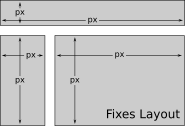
\includegraphics[scale=1.2]{figures/jan/Wire_Fixes-Layout.png}
    \hspace{0.05\textwidth}
    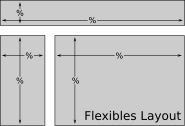
\includegraphics[scale=1.2]{figures/jan/Wire_Flexibles-Layout.png}
    \caption[Aufbau eines fixen und flexiblen Layouts]{Aufbau eines fixen und flexiblen Layouts}
    \label{fig:image}
\end{figure}

Das Gegenstück zum fixen Layout stellt das flexible Layout dar. Dieses passt sich allen Veränderungen unmittelbar an und behält dadurch zu jeder Zeit alle vorgegebenen Größenverhältnisse. Definiert wird es im Gegensatz zu den festen Pixelwerten mit relativen prozentualen Werten, wodurch es sich unterschiedlichen Varianten einer Website leicht anpassen kann. Der reine Layouttyp kommt jedoch eher selten zum Einsatz. Vielmehr lässt sich häufig eine Mischform aus fixem und flexiblem Layout vorfinden.

Eine weitere Layoutform ist das elastische Layout. Das elastische Layout verfolgt den Ansatz, dass sich die Inhalte einer Seite anpassen. Dieser Layouttyp ist besonders für Inhalte geeignet, die die vollständige Bildschirmbreite ausfüllen, was \bspw bei einer Produktpräsentation mit großformatigen Bildern und Videos der Fall ist. Die Inhalte müssen hierfür in der Lage sein sich automatisch flexibel anzupassen. Daher ist es für diese Form von Vorteil, wenn es eher wenige Inhalte zum Vorstellen gibt.

Auf Basis des flexiblen Layouts setzt das responsive Layout auf und erweitert die Möglichkeiten situationsgerecht ein passendes Layout für das Endgerät zur Verfügung zu stellen. Das responsive Layout besitzt als Erweiterung sogenannte Media-Queries, welche es ermöglichen beim Über- oder Unterschreiten fester Schwellwerte eine Veränderung der Ansicht zu starten und die Inhalte \bspw neu anzuordnen.

\subsection{Grundlagen Wireframes}

\subsubsection{Definition/ Inhalte}

Als Wireframe wird die schematische Darstellung von Inhalten und Elementen der Seitenoberfläche verstanden. Wireframes dienen insbesondere zur Konzeptionierung in der Planungsphase, um einerseits einen groben Entwurf für die Verteilung, Anordnung und Gestaltung von den Seitenelementen zu erhalten sowie zum anderen die Beziehungen zwischen den Seiten herzustellen.
Die Darstellung des Seitenlayouts ist zumeist eine skizzenhafte, in schwarz-weiß/ grau gehaltene Abbildung. Die einzelnen Bestandteile der Seite werden dabei durch einfache geometrische Formen verdeutlicht. Das Darstellen von Design, Farben, Schrift und Bilder ist kein Bestandteil der Methode. Ein fertiges Wireframe gibt dem Betrachter final Aufschluss über die Platzierung der Informationsinhalte, die Struktur und Navigation der Seite und die Interaktionselemente (Interface), mit welchen der Nutzer interagiert.
Die ausgearbeiteten Wireframes stellen weiter fort die Grundlage für die visuelle und funktionale Detaillierung des Produktes dar. Anschließende Schritte können \ua das Erstellen von Mockups oder Prototypen sein.

\subsubsection{Arten}

Wireframes werden allgemein in Low-Fidelity- und High-Fidelity-Wireframes unterschieden.
Low-Fidelity-Wireframes (LFW) stellen das klassische Verständnis von Wireframes dar, bei denen der Fokus allein auf dem funktionalen Design liegt. Die Seitenschemas werden mit einfachsten Formen und ohne konkrete Inhalte erstellt.
Die High-Fidelity-Wireframes (HFW) hingegen stellen die nächste Entwicklungsstufe für die Ausarbeitung des Designs dar. In ihr kommen zunehmend mehr und mehr Designkomponenten wie Farben, Typografie, Abstände, Icons, Text, Bilder und Grafiken zum Einsatz. In den Seiten werden zunehmend auch mehr reale Textlängen und Größenverhältnisse der Elemente und Inhalte mit einbezogen.

\begin{figure}
    \centering
    % [//]: # (BILD Beispiel LFW und HFW)
    % https://mentormate.com/blog/low-fidelity-wireframes-vs-high-fidelity-wireframes/
    % https://www.resolutesoftware.com/news/ux-wireframes/
    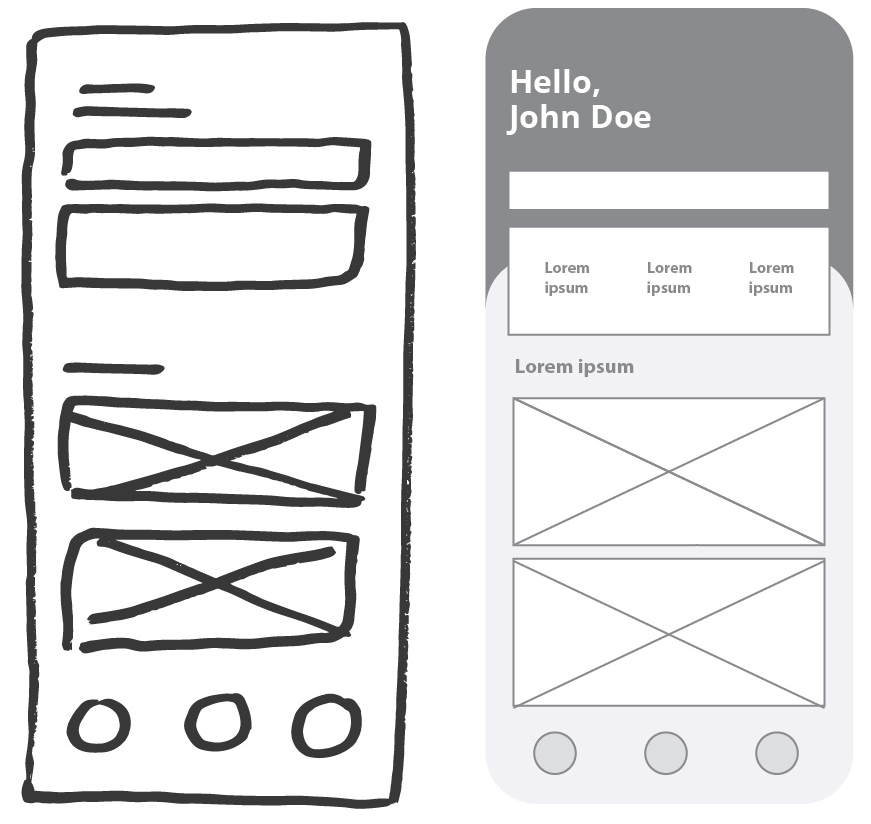
\includegraphics[scale=1]{figures/jan/Wire_Fixes-LFWvsHFW2.png}
    \caption[Beispielhafte Darstellung von LFW und HFW]{Beispielhafte Darstellung von LFW und HFW}
    \label{fig:image}
\end{figure}

\subsubsection{Abgrenzung}

Häufig werden im Zusammenhang mit Wireframes noch weitere visuelle Methoden in Verbindung gebracht. Weit verbreitet sind hier insbesondere Mockups und Prototypen. Diese Methoden verwenden jeweils Wireframes als Grundlage und zielen auf die zunehmende reale Veranschaulichung des zukünftigen Produktes.

Unter Mockups wird das Nachbilden eines Produktes oder auch ein maßstabsgerechtes Modell verstanden. Im Vordergrund der Methode steht das visuell-interaktive Design. Hierzu wird das Konzept der Wireframes übernommen und mit den Elementen der Benutzeroberflächen erweitert. Funktionale oder animierte Elemente sind nicht Bestandteil der Methode und werden nicht für einen Mockup aufgegriffen. Mockups werden im natürlichen Umfeld des Produktes dargestellt - zum Beispiel auf einem Gerätebildschirm. Das Ziel besteht darin das Produkt so echt wie möglich visuell nachzubilden, um dem Kunden ein reales Gefühl über die Erscheinung seines Produktes zu vermitteln.

% \begin{figure}
%     \centering
%     % [//]: # (Bild Mockup in Bildschirm)
%     \includegraphics[scale=0.25]{image.png}
%     \caption[]{image.png}
%     \label{fig:image}
% \end{figure}

Als Prototyp wird ein vereinfachtes Versuchsmodell des geplanten Produktes verstanden. Der Prototyp baut auf die Ergebnisse eines Mockups auf und erweitert dieses mit funktionalen Elementen, um die Interaktion eines Users mit dem Dienst simulieren zu können.
Ein klassisches Beispiel für einen Prototypen ist der Klick-Dummy. Ein Klick-Dummy ist ein teilweise interaktionsfähiges Demo einer Bedienoberfläche, welches alle relevanten Merkmale eines Produktes widerspiegelt und \ua zur Vorstellung oder für Testläufe genutzt werden kann.

\begin{figure}
    \centering
    % https://www.appschopper.com/blog/quick-guide-on-mobile-app-wireframe-vs-mockup-vs-prototype/
    % [//]: # (BILD Reihenfolge LFW - HFW - MockUp - Prototyp)
    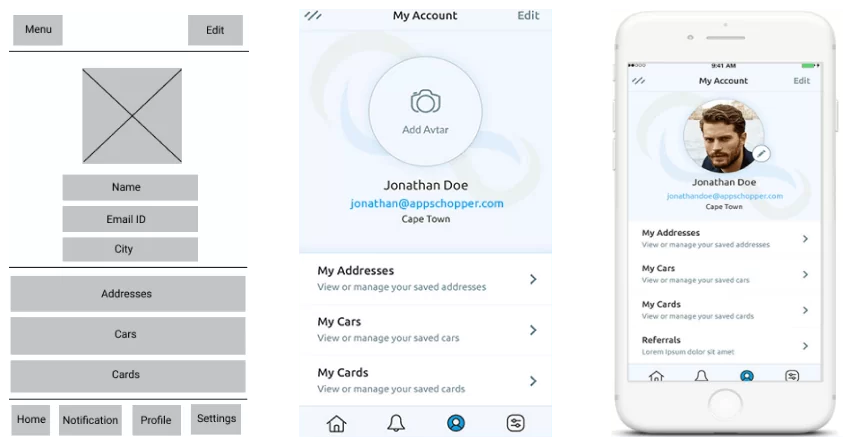
\includegraphics[scale=2]{figures/jan/Wire_Fixes-Wire-prototyp.png}
    \caption[Interationsschritte an einem Beispiel: Wireframe - Mockup - Prototyp]{Interationsschritte an einem Beispiel: Wireframe - Mockup - Prototyp}
    \label{fig:image}
\end{figure}

\subsection{Anwendung}
\subsubsection{Integration}

Die Wireframes wurden innerhalb des Projektverlaufes kontinuierlich für die Ausgestaltung und Kommunikation der User-Stories während des Backlog Refinement verwendet. Hierfür wurden in einer frühen Phase die jeweiligen User-Stories vom PO erläutert und ein erster Wireframe-Entwurf konzipiert. Erkenntnisse, die bereits während der Konzipierung entstanden, wurden an den PO übermittelt und nach Absprache noch während des Sprints direkt in die Wireframes aufgenommen.
Im Refinement dienten sie einerseits dem PO zur Vorstellung und Erklärung der User-Stories und andererseits zur Präzisierung und Detaillierung der Story im Team.
Die daraus neu gewonnenen Informationen wurden vom PO ins Backlog aufgenommen und erneut zum nächsten Refinement in die Wireframes eingearbeitet.

% \begin{figure}
%     \centering
%     % [//]: # (BILD Ablauf: Refinement 0 - 1 - 2 - 3, Feature A, B, C, Iteratives Vorgehen)
%     \includegraphics[scale=0.25]{image.png}
%     \caption[]{image.png}
%     \label{fig:image}
% \end{figure}

Neben der Definition und Veranschaulichung der jeweiligen Features wurden die Wireframes auch im Entwicklungsprozess herangezogen. In diesem wurden sie als gestalterischer Entwurf berücksichtigt und so weit wie es dem Entwickler möglich war, implementiert.

\subsubsection{Auswahl Tool}

Für die Erstellung von Wireframes stehen eine Vielzahl von verschiedenen Softwarelösungen zur Verfügung. Grundsätzlich lassen sich diese in desktop- und webbasierte Anwendungen unterscheiden. Für die Erstellung der Wireframes war es essenziell, dass diese leicht erstellt und angepasst werden können, \ggf auch paralleles Arbeiten möglich ist und dass das Teilen der aktuellen Entwürfe ohne zusätzlichen Aufwand geschieht. Anhand der Basisanforderungen konzentrierte sich die Auswahl zunehmend auf rein webbasierte Lösungen. Als Anbieter kristallisierte sich im weiteren Rechercheverlauf zunehmend Figma als ein passender Dienst heraus.

\begin{figure}
    \centering
    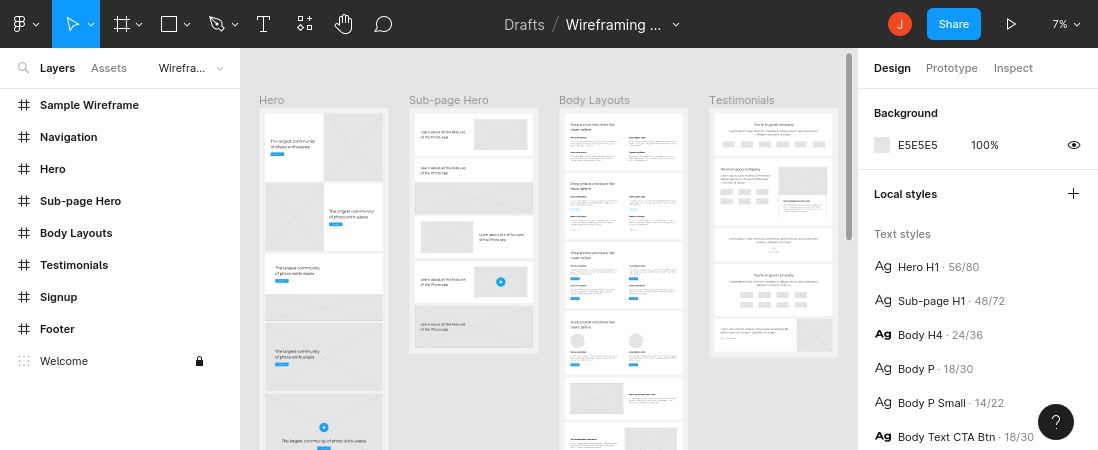
\includegraphics[width=\textwidth]{figures/jan/Wire_Figma.png}
    \caption[Figmas-Arbeitsumgebung]{Figmas-Arbeitsumgebung}
    \label{fig:figma}
\end{figure}

Figma ist eine Onlineanwendung, die sich auf die Erstellung von Wireframes, Mocks und Prototypen spezialisiert und sich in diesem Bereich etabliert hat. Gerade durch die Etablierung des Dienstes lässt sich schließen, dass es als Werkzeug ausgereift ist und die Erstellung einfacher Wireframes durchgängig unterstützt.
Für das Erstellen der Wireframes wurde sich auf die grundlegenden Funktionen von Figma beschränkt. Der verfolgte Ansatz während der Ausarbeitung mit Figma lag hierbei besonders auf der Beschränkung der wesentlichen Elemente, um die Kerninhalte der Features deutlich hervorzuheben. Eingesetzt wurden hierbei \ua zur Gestaltung die Elemente Rechtecke und Text sowie zur Orientierung und Ausrichtung der Inhaltselemente das Raster und die Gruppierfunktion.

\#\#\#\# Anforderungen an die GUI

Für die Ausarbeitung der Wireframes wurden vorab einige Anforderungen festgelegt, welche bei der Erstellung beachtet werden mussten. Die Anforderungen bezogen sich zum einen auf die Gestaltung der Oberfläche und zum anderen auf die technologiekonforme Gestaltung der Wireframes.

Eine wichtige Anforderung an die Plattform war es, die UI generationsübergreifend zu konzipieren. Aus diesem Ansatz heraus ließen sich die folgenden Ansprüche an die UI ableiten:

- Einfache und intuitive Seitengestaltung, um die Inhalte, den Funktionsumfang und die Bedienung schnell selbstständig erfassen zu können,
- Reduzierung der Inhalte auf das Wesentliche, um Verwirrungen/ Ablenkungen zu vermeiden,
- Flache Hierarchien, um direkte Zugriffe auf die gewünschten Inhalte zu ermöglichen.

Von der technologischen Seite her war es erforderlich, dass die erstellten Konzeptentwürfe sich auch mit den ausgewählten Web-Technologien umsetzen lassen. Die Entwickler sollten in die Lage versetzt werden die Entwürfe entweder mittels Eigenentwicklungen oder durch das Heranziehen von Bibliotheken umzusetzen, ohne auf größere Herausforderungen zu stoßen. Das Ziel war es darüber hinaus einen hohen Grad an Wiederverwendbarkeit der Komponenten zu erreichen.

\#\#\#\# Pages

Als geeigneter Wireframetyp wurde ein Hybrid aus LFW und HFW gewählt. Die erstellten Wireframes umfassten alle layouttypischen Bereiche wie Kopf-, Inhalts- und Fußbereich, deren Inhalte in Feldern vereinfacht symbolisiert wurden. Die einzelnen Felder beinhalteten Texte, Dummy-Blöcke \bspw für Bilder und Interaktionselemente (Buttons, Dialoge \usw).
Die Wireframes wurden sehr schlicht in Graustufen gehalten und ohne die Berücksichtigung von Designelementen (Farbe, Typografie \usw) erstellt. Für die regelmäßige Erstellung und Anordnung der Komponenten hat sich nach einigen Entwürfen die Leinwandbreite von 1160 Pixel mit einem Raster von 27×37 Pixel als vorteilhaft ergeben.

Wireframes wurden für die Seiten/ Dialoge

\begin{itemize}
    \item Landingpage,
    \item Registrierung,
    \item Dashboard,
    \item Chat,
    \item Profil,
    \item Accounteinstellungen,
    \item Merkzettel und
    \item Marktplatz
\end{itemize}

erstellt.

Die Art und Detailtiefe der Ausgestaltung zeigen exemplarisch die folgenden Wireframes.

\begin{figure}
    %\centering
    % https://latex.org/forum/viewtopic.php?t=29653
    \begin{minipage}[t]{0.5\textwidth}
        % [//]: # (BILD Wireframes)
        \includegraphics[page=2, width=1\textwidth]{figures/jan/wire_example.pdf}
        \caption[Startseite (DHT)]{Startseite (DHT)}
        \label{fig:image}
    \end{minipage}
    \begin{minipage}[t]{0.5\textwidth}
        % [//]: # (BILD Wireframes)
        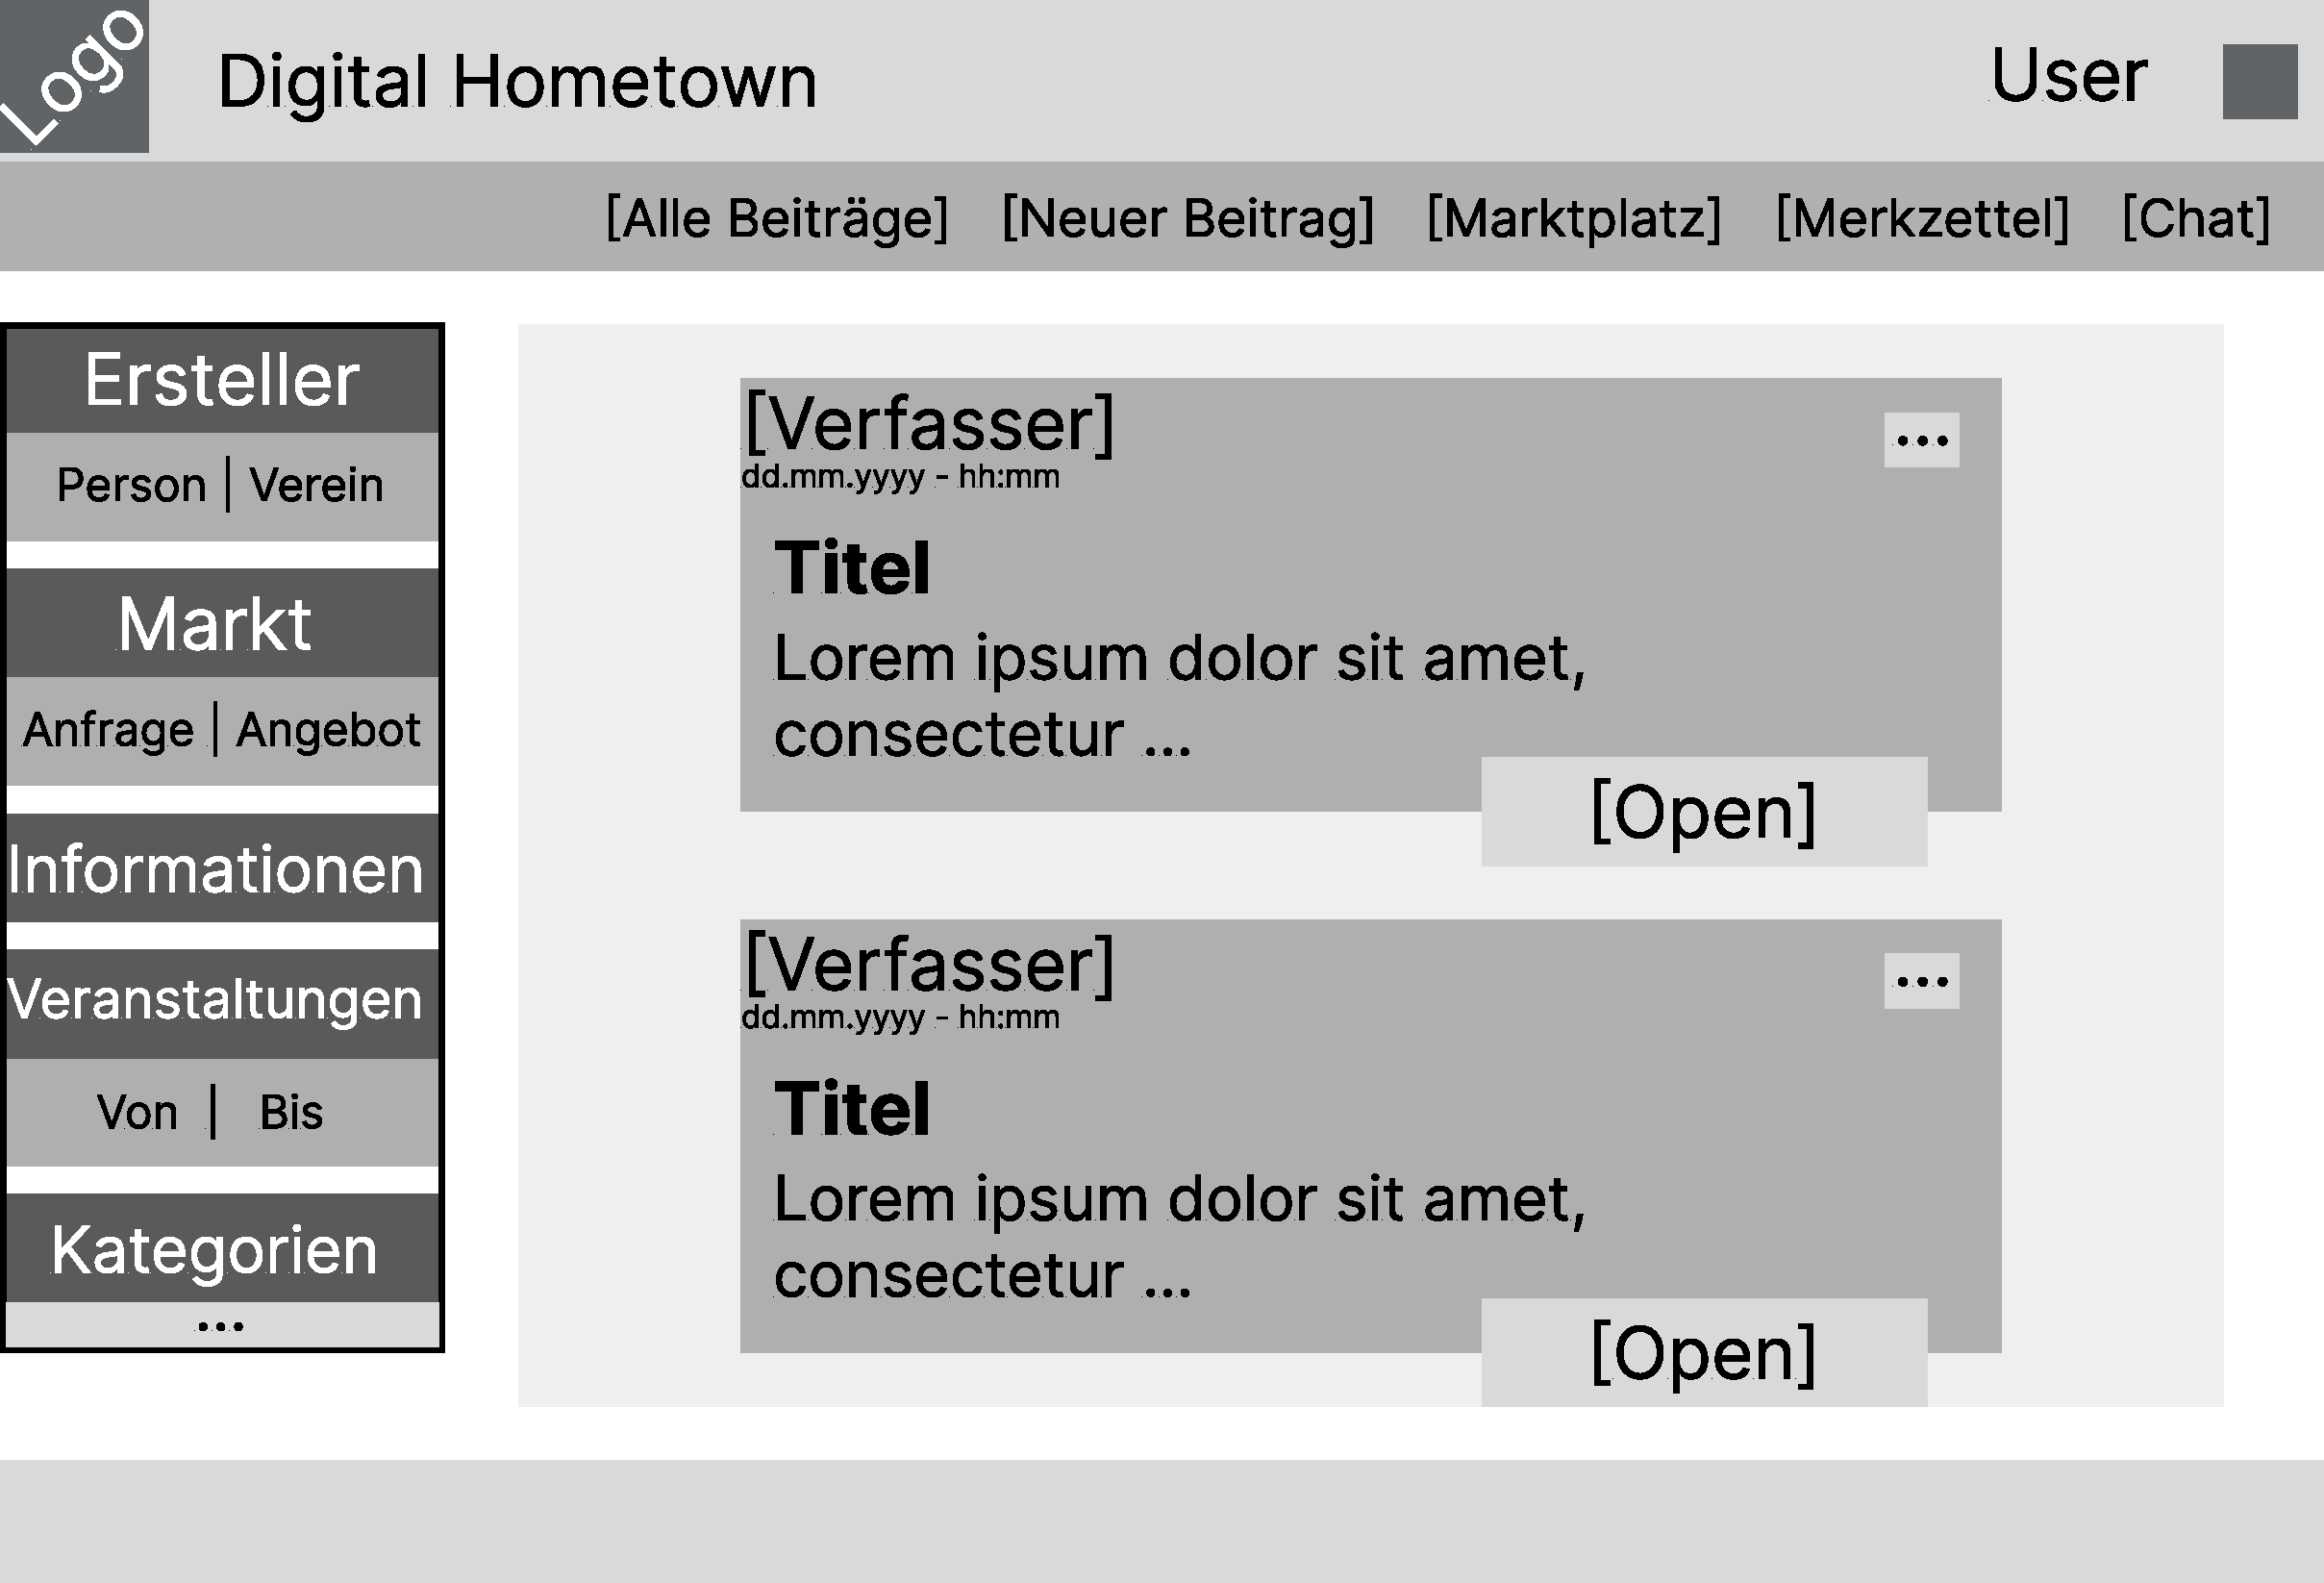
\includegraphics[page=1, width=1\textwidth]{figures/jan/wire_example.pdf}
        \caption[Marktplatz (DHT)]{Marktplatz (DHT)}
        \label{fig:image}
    \end{minipage}
\end{figure}
